\begin{figure}[ht]
    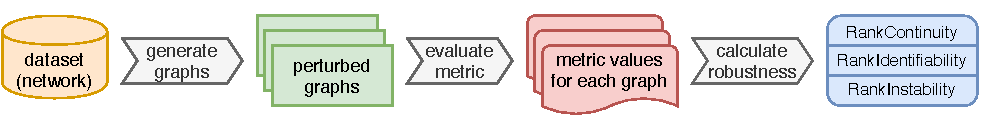
\includegraphics[width=\linewidth]{brief_pipeline.pdf}
    \caption{A brief illustration of the evaluation process.
    A generator is used to generate perturbed graphs from an input dataset.
    A chosen metric is evaluated on all petrurbed graphs, producing per-node values.
    Finally, each robustness measure's value of the metric is calculated.
    This is referred to as the ``Main pipeline'', explained further in \cref{fig:main_data_flow}.}
    \label{fig:brief_pipeline}
\end{figure}
